\documentclass[
    table,
    12pt,
    oneside,
    a4paper,
    italian
]{book}


%pacchetti extra da scaricare dblfloatfix, fancyhdr
\usepackage[left=2cm, right=2cm, bottom=3cm, top=3cm]{geometry}
\usepackage{fancyhdr}%creazione header-footer
\usepackage{graphicx} %serve per inserire immagini
%\graphicspath{ {../../../logo/} }
%\usepackage{dblfloatfix} %serve per posizionare gli elementi dove si vuole
\usepackage[hidelinks]{hyperref} %serve per i link
\usepackage{tikz}
\usepackage{tgadventor} % font
\usepackage[useregional=numeric,showseconds=true,showzone=false]{datetime2}
\usepackage{caption}

\usepackage{hyperref}
\usepackage{tocloft}
\usepackage{titlesec}
\usepackage{color}
\usepackage{ulem}
\usepackage{pgfplots}
\usepackage{pgf-pie}
\usepackage[italian]{babel}
\usepackage{comment}
\usepackage{tabularx}
\usepackage{longtable}
\usepackage{float}
\usepackage{amsmath}

% Load variables
\newcommand{\myName}{Tiozzo Matteo}
\newcommand{\myID}{2042882}
\newcommand{\myTitle}{Decoding GAN-Generated Malware using Explainable AI Techniques}
\newcommand{\myDegree}{Tesi di laurea}
\newcommand{\myUni}{Università degli Studi di Padova}
% For BSc level just use "Corso di Laurea" and don't add "Triennale" to it
\newcommand{\myFaculty}{Corso di Laurea in Informatica}
\newcommand{\myDepartment}{Dipartimento di Matematica ``Tullio Levi-Civita''}
\newcommand{\profTitle}{Prof.}
\newcommand{\myProf}{Alessandro Galeazzi}
\newcommand{\tutorTitle}{Prof.}
\newcommand{\myTutor}{Vinod Puthuvath}
\newcommand{\myLocation}{Padova}
\newcommand{\myAA}{2023-2024}
\newcommand{\myTime}{Dicembre 2024}

% PDF file metadata fields
% when updating them delete the build directory, otherwise they won't change
\begin{filecontents*}{\jobname.xmpdata}
  \Title{Decoding GAN-Generated Malware using Explainable AI Techniques}
  \Author{Tiozzo Matteo}
  \Language{it-IT}
  \Subject{Il presente documento descrive il lavoro svolto durante il periodo di stage, della durata
  complessiva di trecento ore, dal laureando Tiozzo Matteo presso l'Università degli studi di Padova. Il tirocinio è stato condotto sotto la guida del Prof. Alessandro Galeazzi e con la collaborazione del Prof. Vinod Puthuvath. Il Prof. Alessandro Brighente ha
  ricoperto il ruolo di tutor accademico e referente interno al Consiglio del Corso di Studio}
  \Keywords{GAN\sep Malware Analysis}
\end{filecontents*}

% Acronyms
\newacronym{api}{API}{Application Program Interface}
\newacronym{sdk}{SDK}{Software Development Kit}
\newacronym{uml}{UML}{Unified Modeling Language}
\newacronym{tsa}{TSA}{Termine solo acronimo}

% Glossary
\newglossaryentry{apig}{
    name={API},
    text={Application Program Interface},
    sort=api,
    description={In informatics, an API is a set of procedures available to programmers, typically grouped to form a toolkit for a specific task within a program. Its purpose is to provide an abstraction, usually between hardware and the programmer or between low-level and high-level software, simplifying the programming process}
}

\newglossaryentry{sdkg}{
    name={SDK},
    text={Software Development Kit},
    sort=sdk,
    description={A Software Development Kit (SDK) is a collection of development tools in one installable package, facilitating application creation by providing a compiler, debugger, and sometimes a software framework. SDKs are typically specific to a hardware platform and operating system combination. Many application developers use specific SDKs to enable advanced functionalities such as advertisements, push notifications, etc}
}

\newglossaryentry{umlg}{
    name={UML},
    text={Unified Modeling Language},
    sort=uml,
    description={In software engineering, Unified Modeling Language (UML) is a modeling and specification language based on the object-oriented paradigm. UML serves as a "lingua franca" in the object-oriented design and programming community. Much of the industry literature uses UML to describe analytical and design solutions in a concise and understandable way for a broad audience}
}

\newglossaryentry{TermineSenzaAcronimo}{
    name={Nome del termine},
    sort=termine senza acronimo,
    description={Descrizione}
}

% Define custom colors
\definecolor{hyperColor}{HTML}{0B3EE3}
\definecolor{tableGray}{HTML}{F5F5F7}
\definecolor{veryPeri}{HTML}{6667ab}

% Set line height
\linespread{1.5}

% Custom hyphenation rules
\hyphenation {
    data-base
    al-go-rithms
    soft-ware
}

% Images path
\graphicspath{{img/}}

% Force page color, as some editors set a grayish color as default
\pagecolor{white}

% Better spacing for footnotes
\setlength{\skip\footins}{5mm}
\setlength{\footnotesep}{5mm}

\setlength{\headheight}{14.5pt}
\addtolength{\topmargin}{-2.45pt}

% Add a subscript G to a glossary entry
\newcommand{\glox}{\textsubscript{\textbf{\textit{G}}}}

% Improvements the paragraph command
\titleformat{\paragraph}
{\normalfont\normalsize\bfseries}{\theparagraph}{1em}{}
\titlespacing*{\paragraph}
{0pt}{3.25ex plus 1ex minus .2ex}{1.5ex plus .2ex}

% Define use case environment
\newcounter{usecasecounter} % define a counter
\setcounter{usecasecounter}{0} % set the counter to some initial value
% Parameters
% #1: ID
% #2: Nome
\newenvironment{usecase}[2]{
    \renewcommand{\theusecasecounter}{\usecasename #1}  % this is where the display of the counter is overwritten/modified
    \refstepcounter{usecasecounter} % increment counter
    \vspace{2em}
    \par \noindent % start new paragraph
    {\normalsize \textbf{\usecasename #1: #2}} % display the title before the content of the environment is displayed
    \vspace{.5em}
}{
    \medskip
}
\newcommand{\usecasename}{UC}
\newcommand{\usecaseactors}[1]{\textbf{\\Attori Principali:} #1}
\newcommand{\usecasepre}[1]{\textbf{\\Precondizioni:} #1}
\newcommand{\usecasedesc}[1]{\textbf{\\Descrizione:} #1}
\newcommand{\usecasepost}[1]{\textbf{\\Postcondizioni:} #1}
\newcommand{\usecasealt}[1]{\textbf{\\Scenario Alternativo:} #1}

% Define risks environment
\newcounter{riskcounter} % define a counter
\setcounter{riskcounter}{0} % set the counter to some initial value
% Parameters
% #1: Title
\newenvironment{risk}[1]{
    \refstepcounter{riskcounter} % increment counter
    \par \noindent % start new paragraph
    \textbf{\arabic{riskcounter}. #1} % display the title before the content of the environment is displayed
}{
    \par\medskip
}
\newcommand{\riskname}{Rischio}
\newcommand{\riskdescription}[1]{\textbf{\\Descrizione:} #1.}
\newcommand{\risksolution}[1]{\textbf{\\Soluzione:} #1.}

% Apply fancy styling to pages
\pagestyle{fancy}
\fancyhf{}
\fancyhead[L]{\leftmark} % Places Chapter N. Chatper title on the top left
\fancyfoot[C]{\thepage} % Page number in the center of the footer

% Adds a blank page while increasing the page number
\newcommand\blankpage{ 
\clearpage
    \begingroup
    \null
    \thispagestyle{empty}
    \hypersetup{pageanchor=false}
    \clearpage
\endgroup
}

% Adds a blank page while increasing the page number
\newcommand\blankpagewithnumber{ 
  \clearpage
  \thispagestyle{plain} % Use plain page style to keep the page number
  \null
  \clearpage
}

% Increase page numbering
\newcommand\increasepagenumbering{
    \addtocounter{page}{+1}
}

% Make glossaries and bibliography
\makeglossaries
% Redefine the format for the glossary entries to be italic
\renewcommand*{\glstextformat}[1]{\textit{#1}\glox}
%\glsaddall

\bibliography{references/bibliography}
\defbibheading{bibliography} {
    \cleardoublepage
    \phantomsection
    \addcontentsline{toc}{chapter}{\bibname}
    \chapter*{\bibname\markboth{\bibname}{\bibname}}
}

% Code blocks handling w/ table of codes
\makeatletter
\ifdefined\NR@chapter
  \expandafter\@firstoftwo
\else
  \expandafter\@secondoftwo
\fi{\patchcmd\NR@chapter}{\patchcmd\@chapter}
  {\addtocontents{lot}{\protect\addvspace{10\p@}}}
  {\addtocontents{lot}{\protect\addvspace{10\p@}}%
   \addtocontents{lol}{\protect\addvspace{10\p@}}}
  {}{}
\makeatother

\renewcommand\listingscaption{Codice}
\renewcommand\listoflistingscaption{Elenco dei codici sorgenti}
\counterwithin*{listing}{chapter}
\renewcommand\thelisting{\thechapter.\arabic{listing}}

% Set up hyperlinks
\hypersetup{
    colorlinks=true,
    linktocpage=true,
    pdfstartpage=1,
    pdfstartview=,
    breaklinks=true,
    pdfpagemode=UseNone,
    pageanchor=true,
    pdfpagemode=UseOutlines,
    plainpages=false,
    bookmarksnumbered,
    bookmarksopen=true,
    bookmarksopenlevel=1,
    hypertexnames=true,
    pdfhighlight=/O,
    allcolors = hyperColor
}

% Set up captions
\captionsetup{
    tableposition=top,
    figureposition=bottom,
    font=small,
    format=hang,
    labelfont=bf
}

% When draft mode is on, the hyperlinks are removed. Useful when printing the document. To enable/disable, uncomment/comment the command
% \hypersetup{draft}

% prevents cleaning up the cache at the end of the run (needed to keep the unused caches, generated by other editions)
\makeatletter
\renewcommand*{\minted@cleancache}{}
\makeatother

% Break lines in code blocks whe using inputminted
\setminted{breaklines}

\date{}

\hypersetup{pdfstartview=}
\begin{document}
    \frontmatter
    \begin{titlepage}
    \begin{center}
        \begin{Large}
            \textbf{\myUni}\\
        \end{Large}

        \vspace{5pt}

        \begin{large}
            \textsc{\myDepartment}\\
        \end{large}

        \vspace{5pt}

        \begin{large}
            \textsc{\myFaculty}\\
        \end{large}

        \vspace{25pt}
        
        \begin{figure}[htbp]
            \centering
            
\includegraphics[alt={Emblema dell'Università degli Studi di Padova}, height=6cm]{img/logo_unipd.jpeg}
        \end{figure}

        
        \begin{Large}
            \textbf{\myTitle}\\
        \end{Large}

        \vspace{5pt}

        \begin{large}
            \textit{\myDegree}\\
        \end{large}

        \vspace{50pt}
        
        \begin{normalsize}
            \begin{flushleft}
                \textit{Relatore}\\
                \profTitle\ \myProf
            \end{flushleft}

            \vspace{-48pt}
            
            \begin{flushright}
                \textit{\graduateTitle}\\
                \myName\\
                Matricola \myStudentID
            \end{flushright}
        \end{normalsize}

        \vspace*{\fill}
        
        \line(1, 0){338} \\
        \begin{normalsize}
            \textsc{Anno Accademico \myAA}
        \end{normalsize}
    \end{center}
\end{titlepage}

    \increasepagenumbering % increase the page numbrering by 1, in order to cout the frontispiece
    \clearpage
\phantomsection
\thispagestyle{empty}
\hfill
\vfill

{\small\noindent\textcopyright\ \myName, \myTime. Tutti i diritti riservati. \myDegree: ``\textit{\myTitle}'', \myUni, \myDepartment.}
    \cleardoublepage
\phantomsection
\pdfbookmark{Ringraziamenti}{Ringraziamenti}

\begin{flushright}{
    \slshape
    ``Colui il quale ha inseguito e sconfitto i demoni Sem, che ora vagano per il mondo, domandandosi: «ma nü, chi sëm?»''} \\
    \medskip
    --- Il grande Pdor, figlio di Kmer, della tribù di Ishtar, della terra desolata dei Kfnir, uno degli ultimi sette saggi: Pfulur, Galér, Astaparigna, Sùsar, Param, Fusus e Tarìm.
\end{flushright}

\begingroup
\let\clearpage\relax
\let\cleardoublepage\relax
\let\cleardoublepage\relax

\chapter*{Ringraziamenti}

\noindent Desidero esprimere la mia gratitudine al professor \myProf, mio relatore, per l'aiuto e il sostegno che mi ha dato durante la stesura dell'elaborato.

\vspace{0.35cm}

\noindent Vorrei anche ringraziare, con affetto, i miei genitori per il loro sostegno, il grande aiuto e la loro presenza in ogni momento durante gli anni di studio.

\vspace{0.35cm}

\noindent Desidero poi ringraziare i miei amici per i bellissimi anni trascorsi insieme e le mille avventure vissute.

\vspace{0.75cm}

\noindent{\myLocation, \myTime}
\hfill \textit{\myName}

\endgroup

    \cleardoublepage
\phantomsection
\pdfbookmark{Compendio}{Compendio}
\begingroup
\let\clearpage\relax
\let\cleardoublepage\relax
\vspace*{-50pt}
\chapter*{Sommario}
\vspace*{-10pt}
Il presente lavoro di tesi si inserisce nell'ambito dell'analisi e rilevazione di malware, con un particolare focus sull'utilizzo delle Reti Generative Avversarie (GAN) come strumento per migliorare la capacità di rilevamento e comprensione di queste minacce. Durante lo stage curricolare, sono stati affrontati diversi aspetti chiave della ricerca, a partire dalla revisione della letteratura esistente sulle tecniche che combinano le GAN con l'analisi del malware. L'obiettivo primario è stato quello di progettare e sviluppare un sistema di rilevamento del malware basato su tecniche di deep learning, come le Convolutional Neural Networks (CNN), supportate da reti avanzate quali InceptionNet e XceptionNet.

Per addestrare e valutare i modelli, è stato raccolto un dataset curato di eseguibili malware da fonti affidabili come MalwareBazaar e VirusShare, etichettato tramite servizi come VirusTotal e AVClass2. I binari di malware sono stati successivamente convertiti in un formato idoneo per essere utilizzati come input per le GAN. Il modello di rete generativa avversaria sviluppato, ispirato a architetture come DCGAN e WGAN, è stato monitorato tramite metriche chiave come la Fréchet Inception Distance (FID) e la qualità visiva dei campioni generati.

Un ulteriore focus del progetto è stato l’impiego di tecniche di Explainable AI (XAI), come Grad-CAM e Lime, per migliorare la trasparenza e l’interpretabilità del modello di rilevamento. Le analisi effettuate includono una valutazione quantitativa dell'interpretabilità dei modelli e l'esecuzione di un'analisi ablation per determinare l'importanza delle caratteristiche chiave.

Il progetto fornisce contributi significativi sia in termini di innovazione nel campo della rilevazione del malware, sia nell'applicazione delle GAN come strumento per la generazione di malware sintetico e la valutazione della loro efficacia. I risultati ottenuti verranno discussi con i ricercatori coinvolti e saranno oggetto di approfondimento nella relazione finale.

\endgroup


    \cleardoublepage
\pdfbookmark{\contentsname}{tableofcontents}
\setcounter{secnumdepth}{5}
\setcounter{tocdepth}{5}     

\tableofcontents
\clearpage

\begingroup
    \let\clearpage\relax
    \let\cleardoublepage\relax
    \let\cleardoublepage\relax

    % Figures list
    \phantomsection
    \pdfbookmark{\listfigurename}{lof}
    \listoffigures
    \vspace*{8ex}

    % Tables list
    \phantomsection
    \pdfbookmark{\listtablename}{lot}
    \listoftables
\endgroup

\begingroup
    % Code list
    \phantomsection
    \pdfbookmark{\listoflistingscaption}{lol}
    \listoflistings
\endgroup

\cleardoublepage
    \printglossary[type=\acronymtype, title=Acronimi e abbreviazioni, toctitle=Acronimi e abbreviazioni]
    \printglossary[type=main, title=Glossario, toctitle=Glossario]
    \blankpage % example of a blank page that also increases the page couter by 1

    \mainmatter
    \chapter{Introduzione}
\label{chap:introduzione}

\begin{figure}[H]
    \centering
    
\includegraphics[alt={Testo alternativo dell'immagine}, width=1\columnwidth]{img/quantum_entanglement.jpeg}
    \caption{Lorem}
    \label{fig:entanglement}
\end{figure}

% Lorem Figure \ref{fig:entanglement}

% Esempio di utilizzo di un termine nel glossario \gls{api}.

% Esempio di citazione direttamente nel testo \cite{site:agile-manifesto}.

% Esempio di citazione nel piè di pagina \footcite{womak:lean-thinking}.


\section{L'azienda}



\section{L'idea}
% Introduzione all'idea dello stage\footcite{article:spooky}.


\section{Organizzazione del testo}
\begin{description}
    \item[{\hyperref[chap:processi-metodologie]{Il secondo capitolo}}] descrive ...
    
    \item[{\hyperref[chap:descrizione-stage]{Il terzo capitolo}}] approfondisce ...
    
    \item[{\hyperref[chap:analisi-requisiti]{Il quarto capitolo}}] approfondisce ...
    
    \item[{\hyperref[chap:progettazione-codifica]{Il quinto capitolo}}] approfondisce ...
    
    \item[{\hyperref[chap:verifica-validazione]{Il sesto capitolo}}] approfondisce ...
    
    \item[{\hyperref[chap:conclusioni]{Nel settimo capitolo}}] descrive ...
\end{description}

Riguardo la stesura del testo, relativamente al documento sono state adottate le seguenti convenzioni tipografiche:
\begin{itemize}
	\item gli acronimi, le abbreviazioni e i termini ambigui o di uso non comune menzionati vengono definiti nel glossario, situato alla fine del presente documento;
	\item per la prima occorrenza dei termini riportati nel glossario viene utilizzata la seguente nomenclatura: \gls{apig};
	\item i termini in lingua straniera o facenti parti del gergo tecnico sono evidenziati con il carattere \textit{corsivo}.
\end{itemize}

% \begin{listing}[H]

% \caption{Example of code}
% \label{listing:a}
% \end{listing}

\newpage
    \chapter{Processi e metodologie}
\label{chap:processi-metodologie}

\begin{figure}[H]
    \centering
    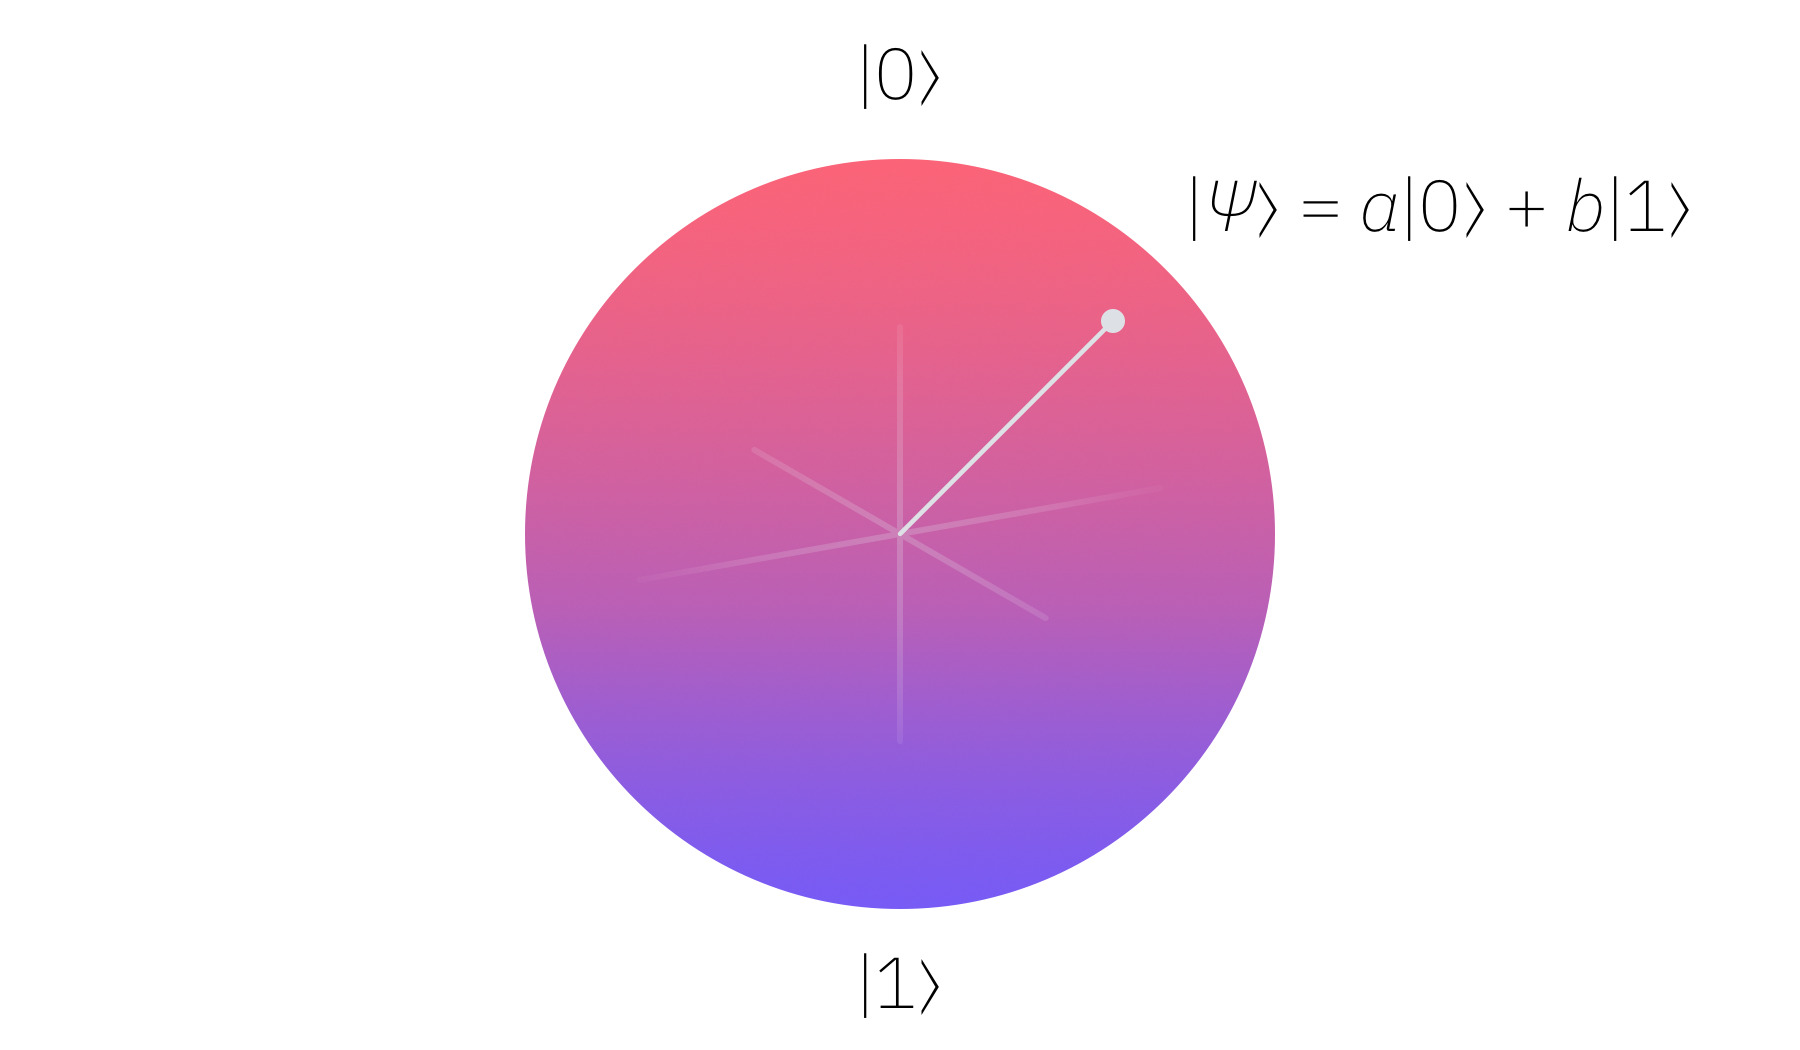
\includegraphics[alt={Testo alternativo dell'immagine}, height=5cm]{img/qubit.jpeg}
    \description[Rappresenzazione Qubit]{Long description}
    \caption{Lorem}
    \label{fig:qubit}
\end{figure}


\section{Processo sviluppo prodotto}


% \begin{listing}[H]

% \caption{Example of code}
% \label{listing:b-2}
% \end{listing}

% Lorem ipsum:
% \begin{listing}[H]

% \caption{Example of code}
% \label{listing:b-3}
% \end{listing}

\newpage
    \chapter{Descrizione dello stage}
\label{chap:descrizione-stage}

\section{Introduzione al progetto}
% \begin{figure}[H] 
%     \centering 
%     
\includegraphics[alt={Testo alternativo dell'immagine}, width=0.5\columnwidth]{img/pk_estate.jpeg}
%     \caption{Caption}
%     \label{fig:pk_estate}
% \end{figure}

\section{Analisi preventiva dei rischi}

% \begin{risk}{Performance del simulatore hardware}
%     \riskdescription{le performance del simulatore hardware e la comunicazione con questo potrebbero risultare lenti o non abbastanza buoni da causare il fallimento dei test}
%     \risksolution{coinvolgimento del responsabile a capo del progetto relativo il simulatore hardware}
%     \label{risk:hardware-simulator} 
% \end{risk}

\section{Requisiti e obiettivi}

% \rowcolors{1}{}{tableGray}
% \begin{longtable}{|p{2.25cm}|p{7.75cm}|p{2.25cm}|}
% \hline
% \multicolumn{1}{|c|}{\textbf{A}} & \multicolumn{1}{c|}{\textbf{B}}\\ 
% \hline 
% \endfirsthead
% \rowcolor{white}
% \multicolumn{3}{c}{{\bfseries \tablename\ \thetable{} -- Continuo della tabella}}\\
% \hline
% \multicolumn{1}{|c|}{\textbf{A}} & \multicolumn{1}{c|}{B}\\ \hline 
% \endhead
% \hline
% \rowcolor{white}
% \multicolumn{3}{|r|}{{Continua nella prossima pagina...}}\\
% \hline
% \endfoot
% \endlastfoot 

% AA & BB \\
% \hline
% AA & BB \\
% \hline
% AA & BB \\
% \hline
% AA & BB \\
% \hline
% \hiderowcolors
% \caption{}
% \label{tab:requisiti_obbiettivi}
% \end{longtable}

\section{Pianificazione}
% \begin{figure}[H]
%     \centering
%     
\includegraphics[alt={Testo alternativo dell'immagine}, width=0.5\columnwidth]{img/pk_estate.jpeg}
%     \caption{Caption}
%     \label{fig:pk_estate_2}
% \end{figure}


\subsection{subsection}


\subsubsection{subsubsection}


\paragraph{paragraph}


\newpage
    \chapter{Analisi dei requisiti}
\label{chap:analisi-requisiti}
    \chapter{Progettazione e codifica}
\label{chap:progettazione-codifica}
% Breve introduzione al capitolo

\section{Tecnologie e strumenti}
\label{sec:tecnologie-strumenti}
% Di seguito viene data una panoramica delle tecnologie e strumenti utilizzati.

% \subsection*{Tecnologia 1}


% \subsection*{Tecnologia 2}

\section{Ciclo di vita del software}
\label{sec:ciclo-vita-software}

\section{Progettazione}
\label{sec:progettazione}

\subsection{Namespace 1}
% Descrizione namespace 1.

\section{Design Pattern utilizzati}

% \section{Codifica}
% Blocco di codice in C
% \begin{listing}[H]
% \begin{minted}{c}
% #include <stdio.h>
% int main() {
%     print("Hello, world!");
%     return 0;
% }
% \end{minted}
% \caption{Example of code}
% \label{listing:c}
% \end{listing}

\newpage
    \chapter{Verifica e validazione}
\label{chap:verifica-validazione}

% \begin{figure}[H]
%     \centering
%     
\includegraphics[alt={Testo alternativo dell'immagine}, width=1\columnwidth]{img/quantum_superposition.jpeg}
%     \caption{Lorem}
%     \label{fig:enter-label}
% \end{figure}

\newpage
    \chapter{Conclusioni}
\label{chap:conclusioni}

\section{Consuntivo finale}
% Esempio di aggiunta di un termine con glossario e acronimo:\\
% Lorem \gls{sdk} ispum dolor.

% Nel successivo utilizzo, apparirà solo l'acronimo:\\
% Lorem \gls{sdk}.

% Nel caso si voglia invece mettere solo il termine per esteso, si può usare:\\
% Lorem \gls{sdkg}.

\section{Raggiungimento degli obiettivi}
% Esempio di termine con solo acronimo\\
% Lorem \gls{tsa}, ipsum dolor sit amet

% termine costruito senza acronimo:
% Lorem \gls{TermineSenzaAcronimo}, ipsum dolor sit amet

\section{Conoscenze acquisite}
% Lorem Ipsum dolor Lorem \gls{api}

% Lorem Ipsum dolor Lorem \gls{apig}

% Si può consultare il file \textit{glossary\_acronyms.tex} per alcuni esempi.

\section{Valutazione personale}


\newpage

    \pagenumbering{roman}
    \backmatter
    \chapter{Bibliografia}
\label{cap:bibliography}

\nocite{*}

% Books bibliography
\printbibliography[heading=subbibliography, title={Testi}, type=book]

% Articles bibliography
\printbibliography[heading=subbibliography, title={Articoli}, type=article]

% Websites bibliography
%\printbibliography[heading=subbibliography, title={Siti}, type=online]

    \chapter{Sitografia}
\label{cap:webliography}
\nocite{*}

% Websites bibliography
\printbibliography[heading=subbibliography, title={\null}, type=online]

\end{document}